\documentclass[tikz,border=6pt]{standalone}
\usepackage{fontspec}\setmainfont{TeX Gyre Heros}
\usetikzlibrary{arrows.meta,positioning}
\definecolor{c64blue}{RGB}{44,41,177}\definecolor{c64lblue}{RGB}{109,106,239}
\definecolor{cpug}{RGB}{120,120,120}
\begin{document}
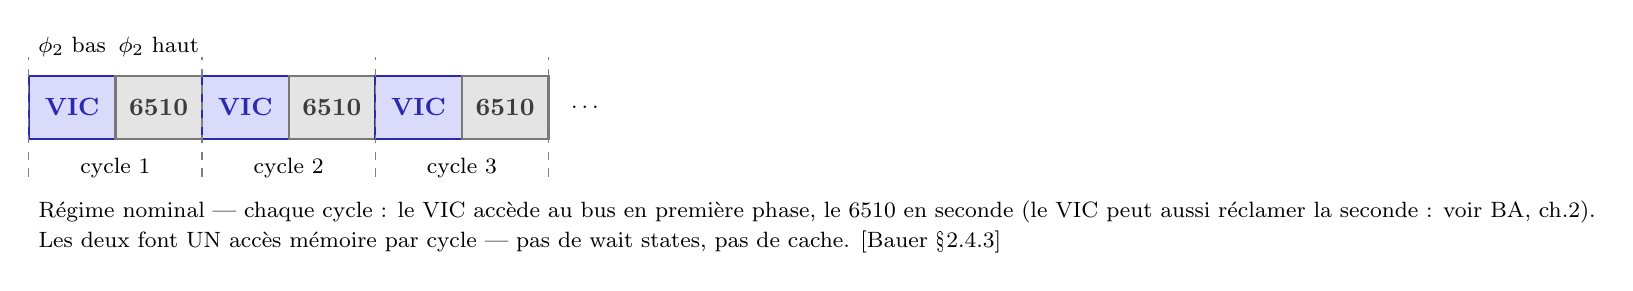
\begin{tikzpicture}[x=1.1cm,y=0.8cm,font=\small]
% trois cycles d'horloge
\foreach \i in {0,1,2}{
  \draw[fill=c64lblue!25,draw=c64blue,thick] (\i*2,0) rectangle ++(1,1);
  \node at (\i*2+0.5,0.5) {\color{c64blue}\textbf{VIC}};
  \draw[fill=cpug!20,draw=cpug,thick] (\i*2+1,0) rectangle ++(1,1);
  \node at (\i*2+1.5,0.5) {\color{cpug!50!black}\textbf{6510}};
  \node[below] at (\i*2+1,-0.15) {\footnotesize cycle \pgfmathparse{int(\i+1)}\pgfmathresult};
  \draw[dashed,gray] (\i*2,-0.6) -- (\i*2,1.3);
}
\draw[dashed,gray] (6,-0.6) -- (6,1.3);
% phase labels
\node[above] at (0.5,1.15) {\footnotesize $\phi_2$ bas};
\node[above] at (1.5,1.15) {\footnotesize $\phi_2$ haut};
\node[right] at (6.15,0.5) {\footnotesize \dots};
\node[align=left,anchor=west] at (0,-1.4) {\footnotesize Régime nominal — chaque cycle : le VIC accède au bus en première
phase, le 6510 en seconde (le VIC peut aussi réclamer la seconde : voir BA, ch.2).\\ \footnotesize Les deux font UN accès mémoire par cycle — pas de wait states,
pas de cache. [Bauer §2.4.3]};
\end{tikzpicture}
\end{document}
